\section{\method}
\label{sec:method}

\begin{wrapfigure}{r}{0.5\textwidth}
\vspace{-4.5em}
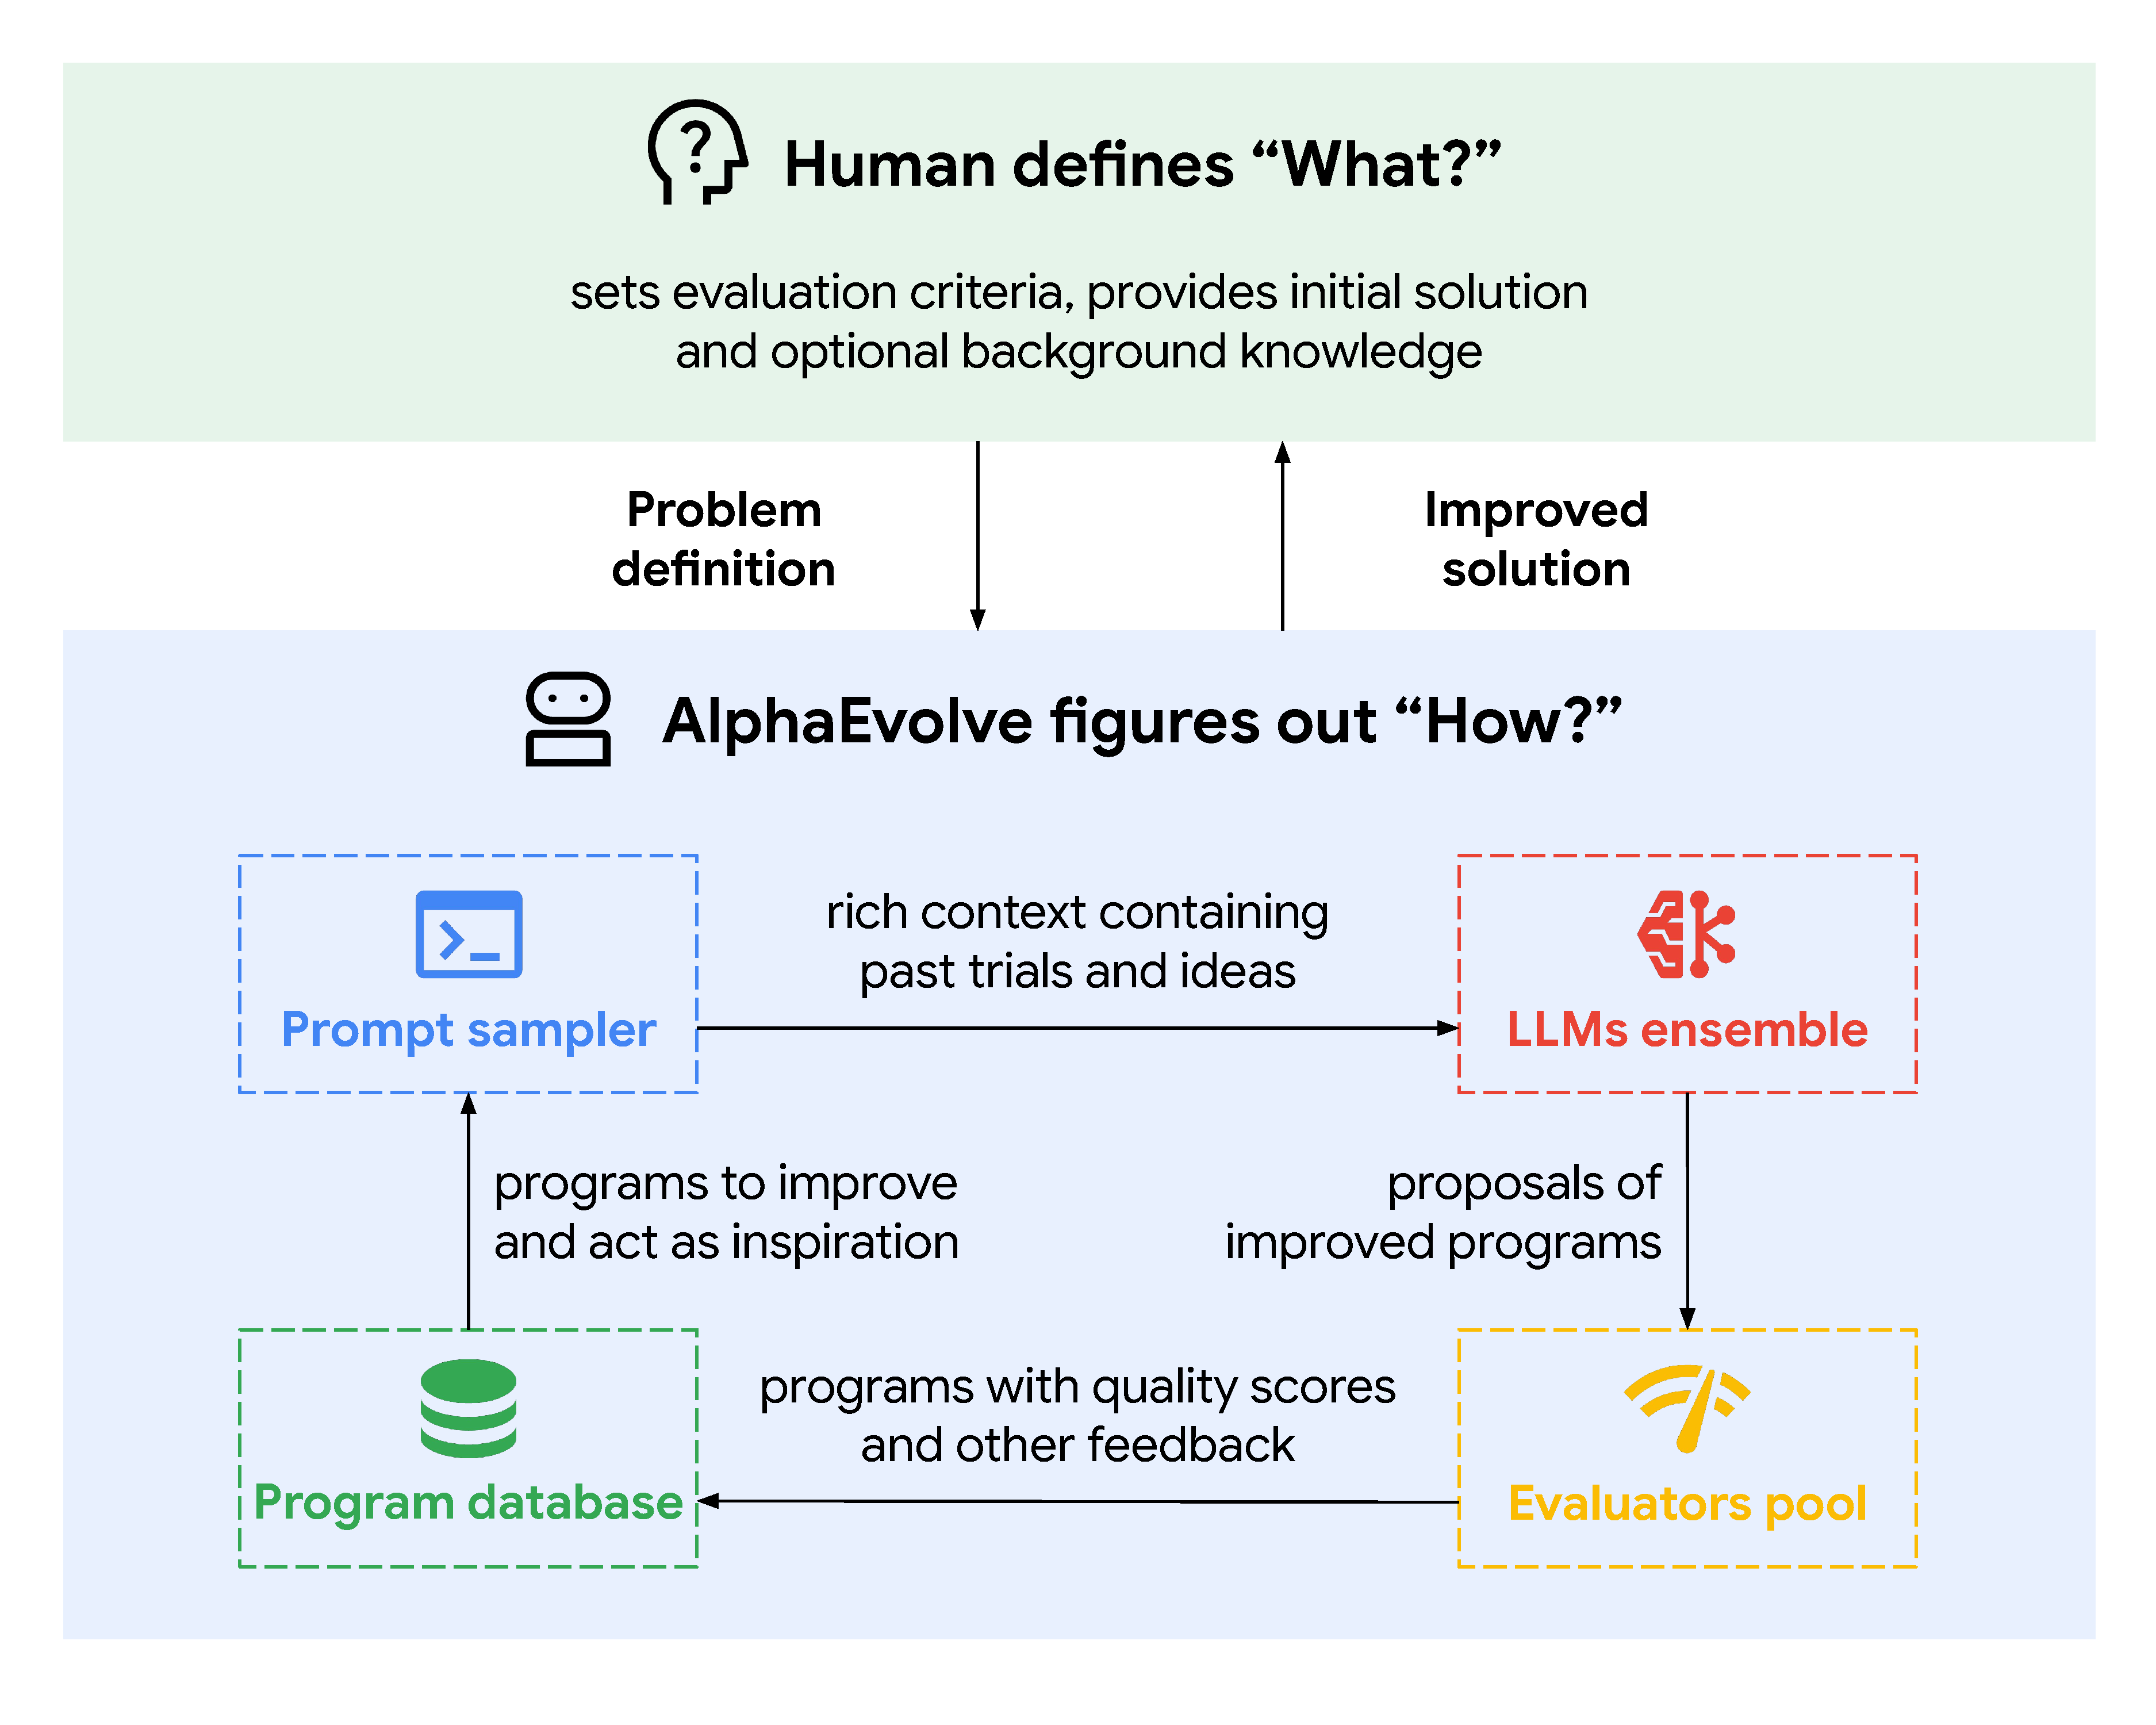
\includegraphics[width=0.99\linewidth, trim=2cm 2cm 2cm 2cm]{figures/method_high_level.pdf}
\caption{\method high-level overview.}
\label{fig:high-level}
\end{wrapfigure}

\method is a coding agent that orchestrates an autonomous pipeline of computations including queries to LLMs, and produces algorithms that address a user-specified task.
At a high level, the orchestrating procedure is an evolutionary algorithm that gradually develops programs that improve the score on the automated evaluation metrics associated with the task.
A high-level overview of \method is shown in~\Cref{fig:high-level}, and~\Cref{fig:method} gives an expanded view.

\begin{figure}[tb]
    \centering
    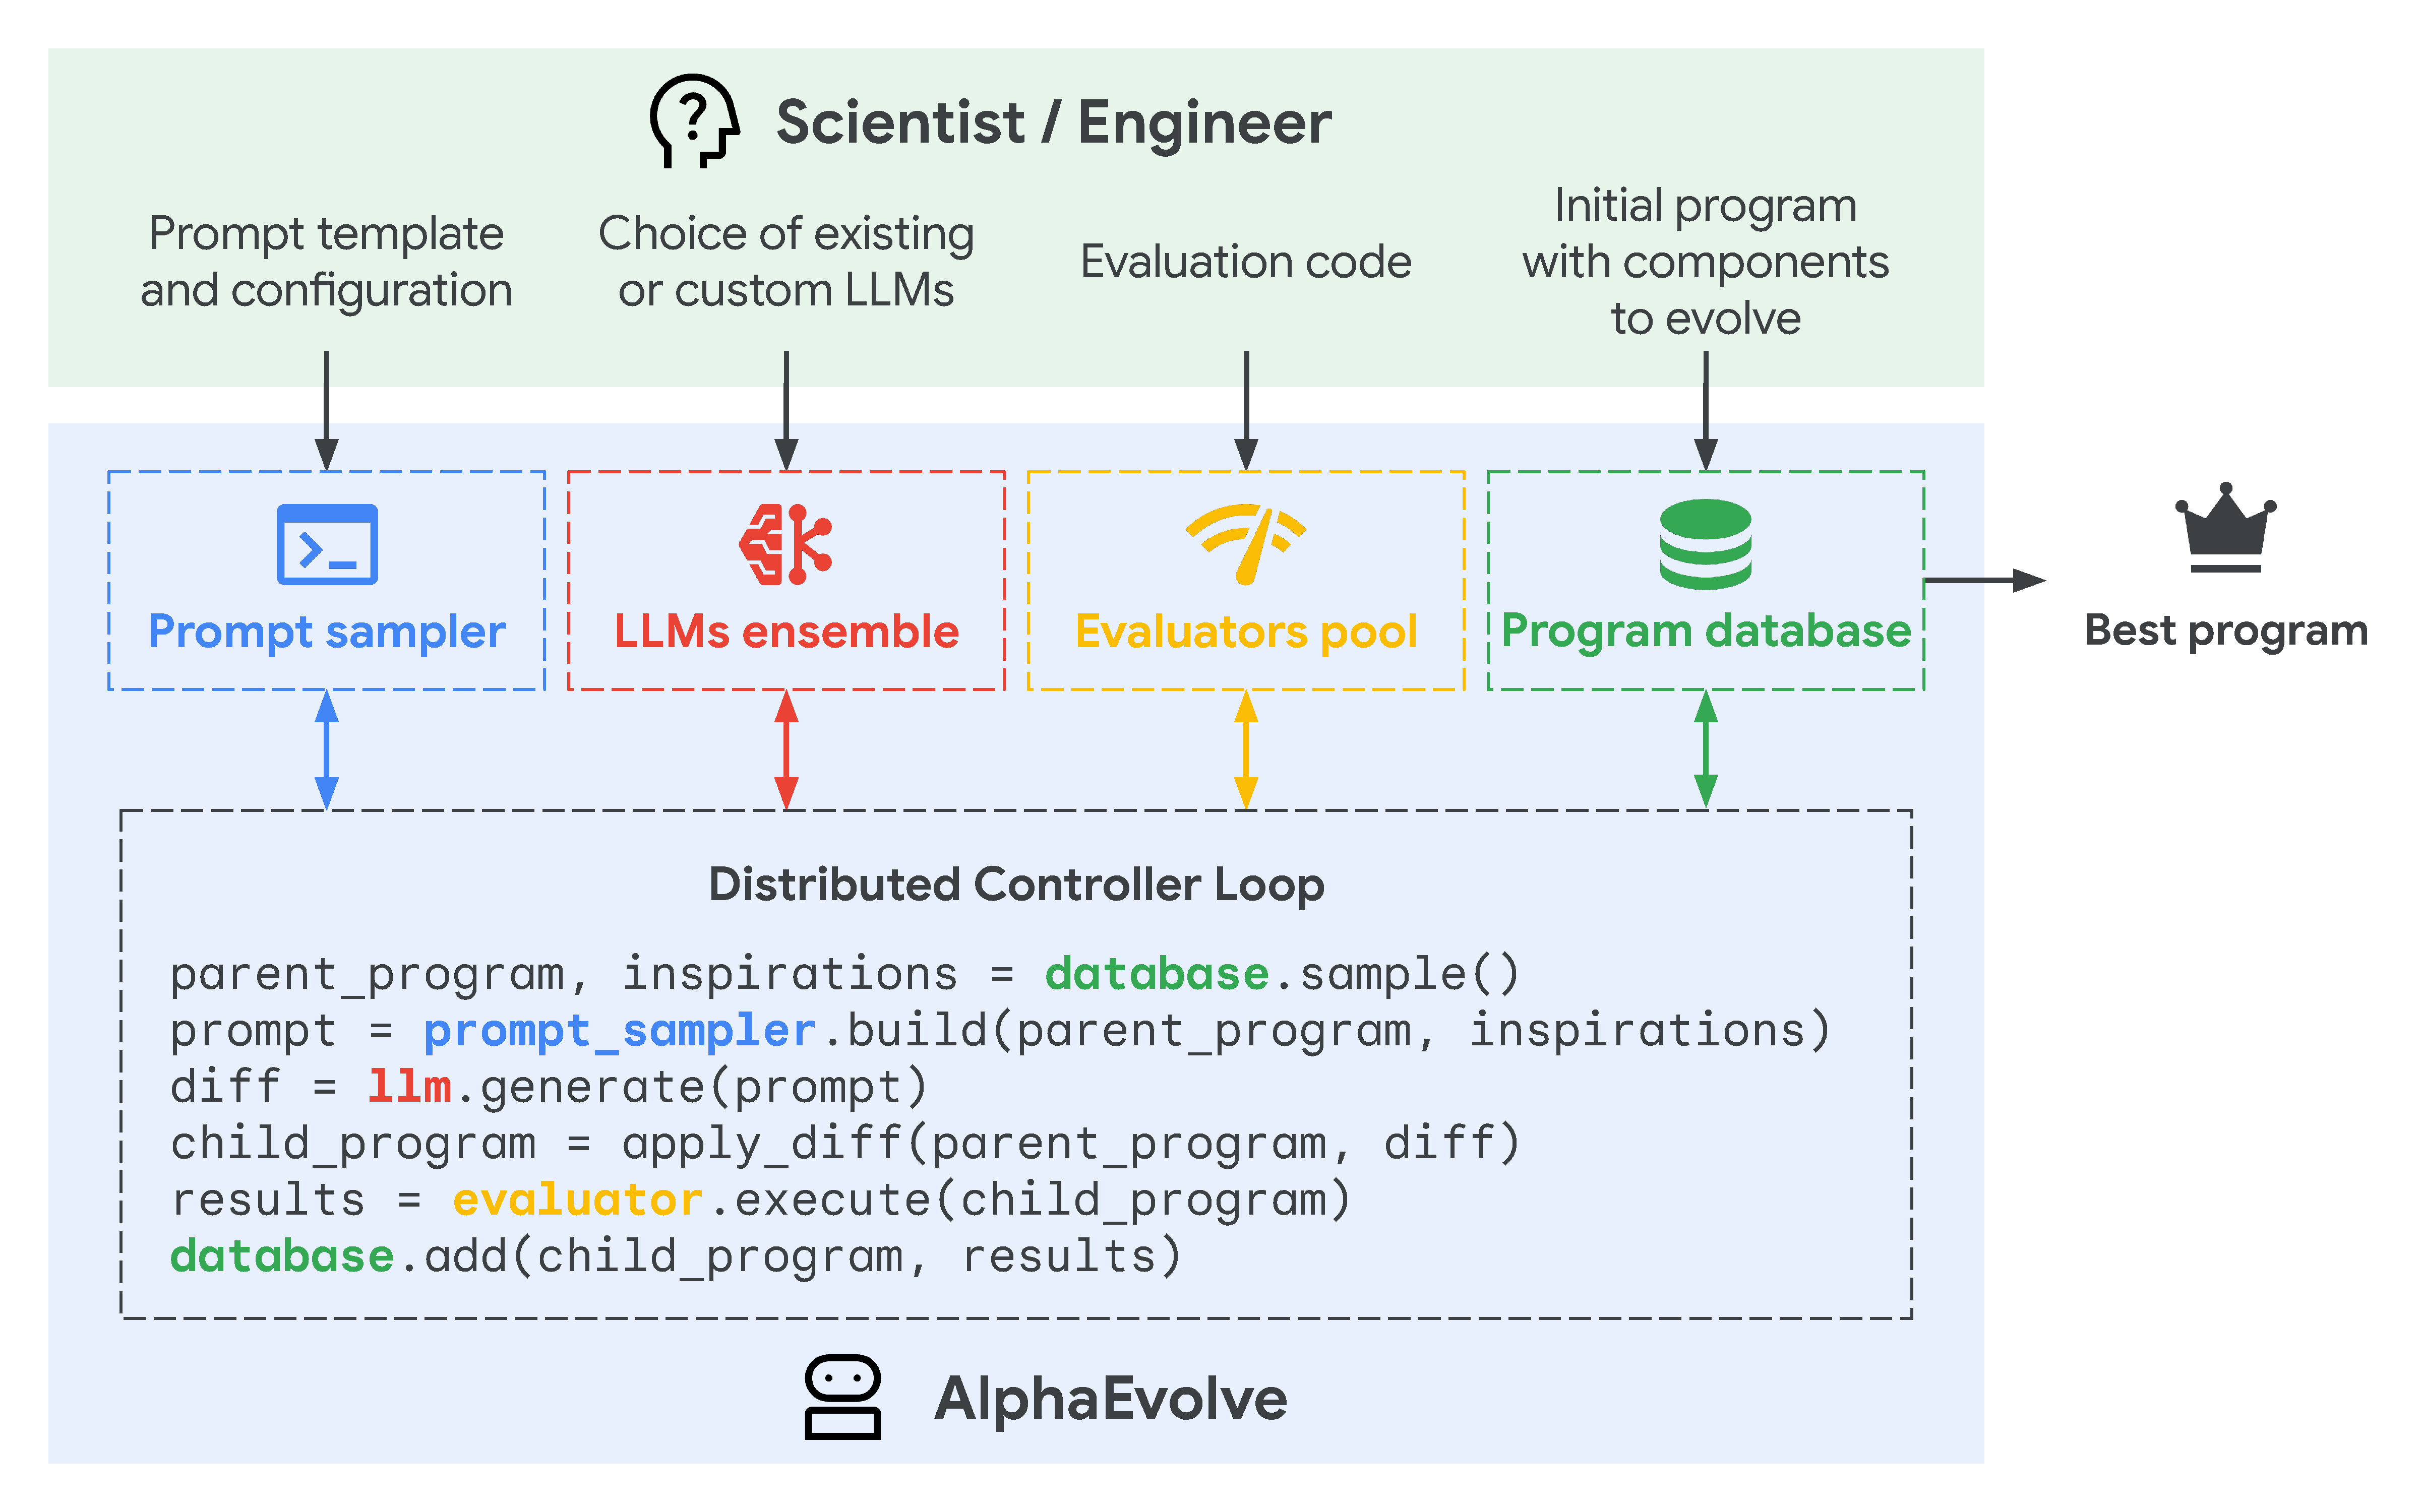
\includegraphics[width=0.96\textwidth, trim=0cm 0cm 0cm 0cm, clip]{figures/method_detailed.pdf}
    \caption{%
    Expanded view of the \method discovery process. The user provides an initial program (with components to evolve marked), evaluation code, and optional configurations (\Cref{subsec:specification}).
    \method then initiates an evolutionary loop.
    The \emph{Prompt sampler} uses programs from the \emph{Program database} to construct rich prompts (\Cref{subsec:prompting}).
    Given these prompts, the \emph{LLMs} generate code modifications (diffs), which are applied to create new programs (\Cref{subsec:generation}).
    These are then scored by \emph{Evaluators} (\Cref{subsec:evaluation}), and promising solutions are registered back into the \emph{Program database} (\Cref{subsec:evolution}), driving the iterative discovery of better and better programs.
    }
    \label{fig:method}
\end{figure}


\subsection{Task specification}
\label{subsec:specification}

\paragraph{Evaluation.} Since \method tackles problems with machine-gradeable solutions, the user must provide a mechanism for automatically assessing generated solutions.
This mechanism takes the form of a function $h$ mapping a solution to a set of scalar evaluation metrics.
By convention, these metrics are maximized.
In our current setup, $h$ is typically implemented as a Python function, called \texttt{evaluate}, with a fixed input/output signature, returning a dictionary of scalars.

Depending on the application, executing this function may take only seconds on a single device or spawn extensive computations. For mathematical problems, the function $h$ is typically very simple.
For example, when wishing to find largest possible graphs satisfying a given property, $h$ invokes the evolved code to generate a graph, checks whether the property holds, and then simply returns the size of the graph as the score.
In more complicated cases, the function $h$ might involve performing an evolved search algorithm, or training and evaluating a machine learning model.

\paragraph{API.} To support evolving multiple components across a codebase, \method exposes an input API where blocks of code can be annotated as to-be-evolved-by-the-system; see Figure~\ref{fig:grounding-api} for an illustration. This design facilitates integrating it with existing codebases while requiring only minimal changes, simply by adding special markers (\texttt{\# EVOLVE-BLOCK-START} and \texttt{\# EVOLVE-BLOCK-END}) as comments into the code.

Any user-provided code inside such evolution blocks serves as the initial solution to be improved by \method, and the rest of the code forms a skeleton that ties the evolved pieces together, so that they can be invoked from \texttt{evaluate}. 
While this initial implementation must be complete, it can be rudimentary---for instance, consisting of single-line functions that return constants of the appropriate types.

\begin{figure}[htbp]
    \centering
    \begin{minipage}[c]{0.48\textwidth} %
        \centering
        \begin{subfigure}[t]{\textwidth} %
            \centering
\begin{minted}[fontsize=\tiny, bgcolor=backcolour]{python}
# EVOLVE-BLOCK START
"""Image classification experiment in jaxline."""

import jax
...
# EVOLVE-BLOCK-END

...

# EVOLVE-BLOCK-START
class ConvNet(hk.Module):
  def __init__(self, num_classes): ...
  def __call__(self, inputs, is_training): ...


def sweep():
  return hyper.zipit([...])
# EVOLVE-BLOCK-END

...

def evaluate(eval_inputs) -> dict[str, float]:
  ...
  return metrics
\end{minted}
            \captionsetup{justification=centering, singlelinecheck=false}
            \caption{\raisebox{-0.3\baselineskip}{
\includegraphics[height=1.8em]{assets/human-icon.png}}}
            \label{fig:grounding-api}
        \end{subfigure}
        \vfill %
        \begin{subfigure}[b]{\textwidth} %
            \centering

\begin{minted}[fontsize=\tiny, bgcolor=backcolour, escapeinside=||, breaksymbolleft={}]{python}
|The current model uses a simple ResNet architecture with only three ResNet blocks. We can improve its performance by increasing the model capacity and adding regularization. This will allow the model to learn more complex features and generalize better to unseen data. We also add weight decay to the optimizer to further regularize the model and prevent overfitting. AdamW is generally a better choice than Adam, especially with weight decay.|


<<<<<<< SEARCH
    self._block1 = ResNetBlock(num_channels)
    self._block2 = ResNetBlock(num_channels * 2, stride=2)
    self._block3 = ResNetBlock(num_channels * 4, stride=2)
=======
    self._block1 = ResNetBlock(num_channels)
    self._block2 = ResNetBlock(num_channels, stride=1)
    self._block3 = ResNetBlock(num_channels * 2, stride=2)
    self._block4 = ResNetBlock(num_channels * 2, stride=1)
    self._block5 = ResNetBlock(num_channels * 4, stride=2)
    self._block6 = ResNetBlock(num_channels * 4, stride=1)
>>>>>>> REPLACE
<<<<<<< SEARCH
  def optimizer(self, learning_rate):
    return optax.adam(learning_rate)
=======
  def optimizer(self, learning_rate):
    return optax.adamw(learning_rate, weight_decay=1e-4)
>>>>>>> REPLACE
\end{minted}
            \addtocounter{subfigure}{+1}
            \captionsetup{justification=centering, singlelinecheck=false}
            \caption{\raisebox{-0.5\baselineskip}{
\includegraphics[height=2.0em]{assets/llm-icon.png}}}
            \label{fig:grounding-llm}
        \end{subfigure}
    \end{minipage}
    \hfill %
    \begin{minipage}[c]{0.48\textwidth} %
        \centering
        \begin{subfigure}{\textwidth} %
            \centering

\begin{minted}[fontsize=\tiny, bgcolor=backcolour, escapeinside=||, breaksymbolleft={}]{python}
|Act as an expert software developer. Your task is to iteratively improve the provided codebase. [...]

- Prior programs

Previously we found that the following programs performed well on the task at hand:|

top_1_acc: 0.796; neg_eval_log_loss: 0.230; average_score: 0.513

"""Image classification experiment in jaxline."""
[...]
class ConvNet(hk.Module):
  """Network."""

  def __init__(self, num_channels=32, num_output_classess=10):
    super().__init__()
    self._conv1 = hk.Conv2D(num_channels, kernel_shape=3)
    self._conv2 = hk.Conv2D(num_channels * 2, kernel_shape=3)
    self._conv3 = hk.Conv2D(num_channels * 4, kernel_shape=3)
    self._logits_module = hk.Linear(num_output_classes)
[...]


|- Current program

Here is the current program we are trying to improve (you will need to propose a modification to it below).|

top_1_acc: 0.862; neg_eval_log_loss: 0.387; average_score: 0.624

"""Image classification experiment in jaxline."""
[...]
class ConvNet(hk.Module):
  """Network."""

  def __init__(self, num_channels=32, num_output_classes=10):
    super().__init__()
    self._conv1 = hk.Conv2D(num_channels, kernel_shape=3)
    self._block1 = ResNetBlock(num_channels)
    self._block2 = ResNetBlock(num_channels * 2, stride=2)
    self._block3 = ResNetBlock(num_channels * 4, stride=2)
    self._logits_module = hk.Linear(num_output_classes)
|[...]

SEARCH/REPLACE block rules:
[...]

Make sure that the changes you propose are consistent with each other. For example, if you refer to a new config variable somewhere, you should also propose a change to add that variable.

Example:
[...]

Task
Suggest a new idea to improve the code that is inspired by your expert knowledge of optimization and machine learning.  

Describe each change with a SEARCH/REPLACE block.|
\end{minted}
            \addtocounter{subfigure}{-2}
            \captionsetup{justification=centering, singlelinecheck=false}
            \caption{\raisebox{-0.5\baselineskip}{
\includegraphics[height=2.0em]{assets/prompt-icon.png}}}
            \label{fig:grounding-prompt}
        \end{subfigure}
    \end{minipage}
    \caption{Illustrative example of applying \method to evolving a supervised learning pipeline. All snippets are abbreviated, with ellipsis (...) indicating skipped lines. (a) The user-provided file with blocks marked for evolution, and the special \texttt{evaluate} function that can be invoked to score the current version of the code. (b) Example of an assembled prompt to be provided to the LLMs. (c) Example output generated by the LLM. The proposed diffs in (c) will be applied to the "current program" shown in the prompt (b), and the resulting modified program will then be sent to the evaluators. The evaluators will invoke the \texttt{evaluate} function from (a) in order to obtain the scores of the newly proposed program.}
    \label{fig:grounding}
\end{figure}

\paragraph{Flexibility in choosing the abstraction.} \method can be applied to the same problem in very different ways---especially when the evolved programs are not the final output but a means to discover solutions.
For example, \method can evolve the solution in raw string representation (as in classical evolutionary algorithms); evolve a function of a definite form that specifies how to construct the solution from scratch (the approach taken in~\cite{paredes2023mathematical}); evolve a bespoke search algorithm to find the solution within some fixed compute budget; or even co-evolve intermediate solutions and search algorithms together, such that each search algorithm is specifically tailored to further improve upon a particular intermediate solution.

We find that different levels of abstraction work better for different problems.
For example, we hypothesize that for problems with highly symmetric solutions it is advantageous to evolve constructor functions as these tend to be more concise~\cite{paredes2023mathematical}, whereas for problems with non-symmetric solutions it works better to evolve customized search algorithms.


\subsection{Prompt sampling}
\label{subsec:prompting}

As \method leverages SOTA LLMs, it supports various types of customization and providing long contexts as part of the primary evolution prompt.
This prompt comprises multiple previously discovered solutions sampled from the program database, as well as system instructions on how to propose changes to a particular solution.
Beyond these key ingredients, users can further tailor prompts to their specific needs in different ways, such as the following.
\begin{itemize}
\item
\emph{Explicit context}: details about the problem being solved, such as fixed human-written instructions, equations, code snippets, or relevant literature (e.g., pdf files).
\item
\emph{Stochastic formatting}: template placeholders with human-provided alternatives for increased diversity, instantiated using probability distributions provided in a separate config file.
\item
\emph{Rendered evaluation results}: usually this will include a program, the result of executing that program, and the scores assigned by the \texttt{evaluate} function.
\item
\emph{Meta prompt evolution}: instructions and context suggested by the LLM itself in an additional prompt-generation step, co-evolved in a separate database analogous to the solution programs.
\end{itemize}


\subsection{Creative generation}
\label{subsec:generation}

To drive the evolutionary procedure, \method leverages the capabilities of SOTA LLMs, whose principal role is to digest information about previously developed solutions and propose new, diverse ways to improve the solutions.
Although \method is model-agnostic, in ablations we observe that \method performs increasingly better as the underlying LLM improves (see~\Cref{sec:ablations_rewrite}).


\paragraph{Output format.}
When \method asks an LLM to modify existing code, especially within larger codebases, it requests the changes to be provided as a sequence of diff blocks in a specific format:

\begin{verbatim}
<<<<<<< SEARCH
  # Original code block to be found and replaced
=======
  # New code block to replace the original
>>>>>>> REPLACE
\end{verbatim}

Here, the code between \texttt{<{}<{}<{}<{}<{}<{}< SEARCH} and \texttt{=======} is the exact segment to match in the current program version. The code between \texttt{=======} and \texttt{>{}>{}>{}>{}>{}>{}> REPLACE} is the new segment that will replace the original one.
This allows for targeted updates to specific parts of the code.

In cases where the code being evolved is very short, or when a complete rewrite is more appropriate than a small modification, \method can be configured to instruct the LLM to output the entire code block directly, rather than using the diff format. 

\paragraph{Models used.}
\method employs an ensemble of large language models. Specifically, we utilize a combination of Gemini 2.0 Flash and Gemini 2.0 Pro.
This ensemble approach allows us to balance computational throughput with the quality of generated solutions.
Gemini 2.0 Flash, with its lower latency, enables a higher rate of candidate generation, increasing the number of ideas explored per unit of time.
Concurrently, Gemini 2.0 Pro, possessing greater capabilities, provides occasional, higher-quality suggestions that can significantly advance the evolutionary search and potentially lead to breakthroughs.
This strategic mix optimizes the overall discovery process by maximizing the volume of evaluated ideas while retaining the potential for substantial improvements driven by the more powerful model.


\subsection{Evaluation}
\label{subsec:evaluation}

To track \method's progress and to select which ideas to propagate in future generations, each new solution proposed by the LLMs is automatically evaluated.
In principle, this process amounts to simply executing the user-provided evaluation function $h$ on the generated solution.
In practice, \method supports optional mechanisms to make this evaluation more flexible and more efficient:
\begin{itemize}
\item
\emph{Evaluation cascade (hypothesis testing)}: the user can specify ensembles of test cases of increasing difficulty, such that new solutions are  evaluated on the next stage only if they achieve sufficiently promising results in all earlier stages.
This helps to prune out less promising solutions more quickly. Moreover, new solutions are initially evaluated on a small scale before being subjected to the main test cases, to filter out faulty programs early.
\item
\emph{LLM-generated feedback}: in some applications, desirable solutions have certain characteristics that are difficult to capture precisely in the user-provided evaluation function $h$; for example, simplicity of the discovered program.
These properties can be graded using separate LLM calls and added to the dictionary of scores to steer evolution, or they can be used to discard solutions when a criterion is not fulfilled.
\item
\emph{Parallelized evaluation}: the sample efficiency of \method makes it feasible to spend on the order of 100 compute-hours to evaluate any new solution.
However, unless individual evaluations are parallelized to reduce their wall-clock duration, this can slow down the rate at which new generations appear, limiting the ability of the evolutionary algorithm to apply several consecutive mutations.
In many applications, evaluation is embarrassingly parallel (for example, running a search algorithm from multiple randomized initializations), allowing \method to distribute this work through asynchronous calls to an evaluation cluster.
\end{itemize}

\paragraph{Multiple scores.}
\method allows for optimizing multiple user-provided scores, i.e., evolving objects that achieve a high score under one or multiple evaluation metrics.
This has both an intrinsic and instrumental value. While in multiple applications we genuinely care about developing solutions for multiple evaluation metrics (or one solution that is strong on all of them simultaneously), we find that even if one metric is of particular interest, optimizing for multiple metrics often improves results for the single target metric.
Perhaps this occurs because programs excelling under different evaluation criteria often possess distinct structures or logic and, by incorporating examples of these diverse, high-performing programs---each representing a different definition of ``good''---into the prompts provided to the language model, we can stimulate the generation of more varied candidate solutions, increasing the chances of discovering novel approaches that are highly effective for the target metric.


\subsection{Evolution}
\label{subsec:evolution}

During its evolutionary procedure, \method continually generates a growing number of solutions with evaluation results (scores and program outputs) attached to them.
These solutions are stored in an evolutionary database, the primary goal of which is to optimally resurface previously explored ideas in future generations.
A key challenge in designing such databases is balancing exploration and exploitation, to continuously improve the best programs while maintaining diversity to encourage exploration of the entire search space.
In \method, the evolutionary database implements an algorithm that is inspired by a combination of the MAP elites algorithm~\cite{mouret2015illuminating} and island-based population models~\cite{tanese1989distributed, paredes2023mathematical}.


\subsection{Distributed pipeline}
\label{subsec:pipeline}

\method is implemented as an asynchronous computational pipeline (using the \texttt{asyncio} Python library) in which many computations are run concurrently, with each computation blocking (waiting) whenever its next step relies on the result of another, yet unfinished computation.
More specifically, the asynchronous pipeline comprises a controller, LLM samplers, and evaluation nodes.
The entire pipeline is optimized for throughput (rather than the speed of any one particular computation), in order to maximize the number of ideas that can be proposed and evaluated within a specific overall computation budget.
